% ------------------------------------------------------------
\section{Calendar Week}
% ------------------------------------------------------------
% --------------------------------------------------- Slide --
\subsection{CW 42}
% ------------------------------------------------------------
\begin{frame}
  \frametitle{Review CW 42}
	\begin{itemize}
		\item Finished fatigue calculation for test case, now with different cases (i.e., increasing beam (simplified implant)) length due to peri-implantitis. See next slides for a few figures of the results. \textcolor{green}{Done}
	\end{itemize}
\end{frame}

\begin{frame}
  \frametitle{Review CW 42 - Model}
	\begin{figure}
		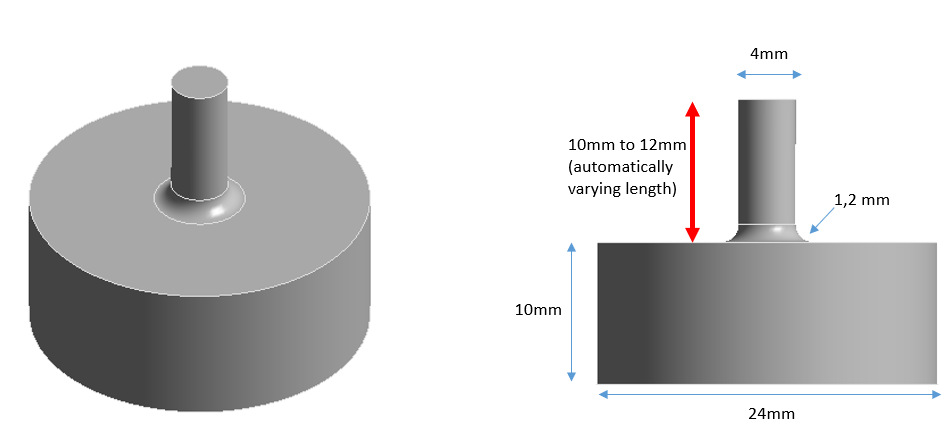
\includegraphics[width=0.8\textwidth]{pictures/CW42_1}
	\end{figure}
	\centering Main dimensions of (very) simplified implant model as a simple cantilever beam.
\end{frame}

\begin{frame}
  \frametitle{Review CW 42 - Material}
	\begin{figure}
		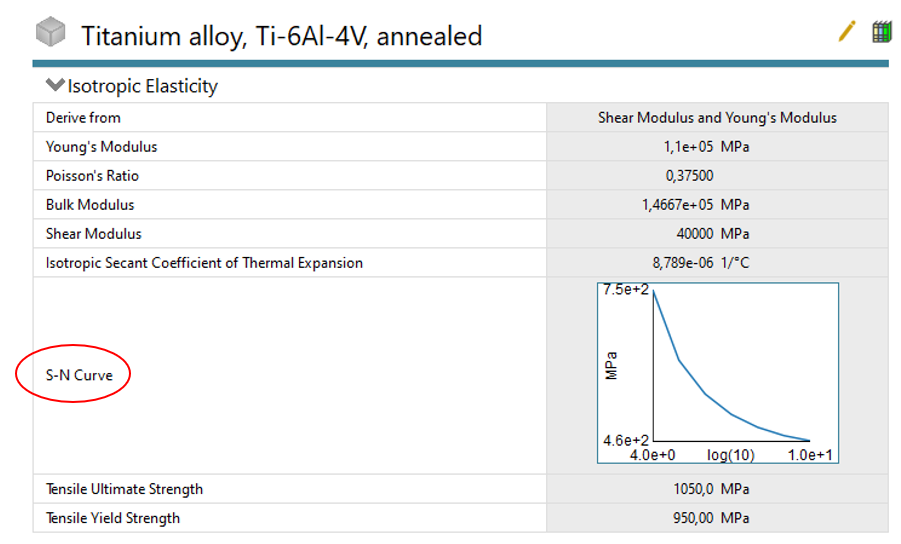
\includegraphics[width=0.8\textwidth]{pictures/CW42_2}
	\end{figure}
	\centering Material (Ti6Al4V) considered. Note SN ("Woehlers) fatigue curve (taken from literature (Janecek2015)).
\end{frame}

\begin{frame}
  \frametitle{Review CW 42 - Mesh}
	\begin{figure}
		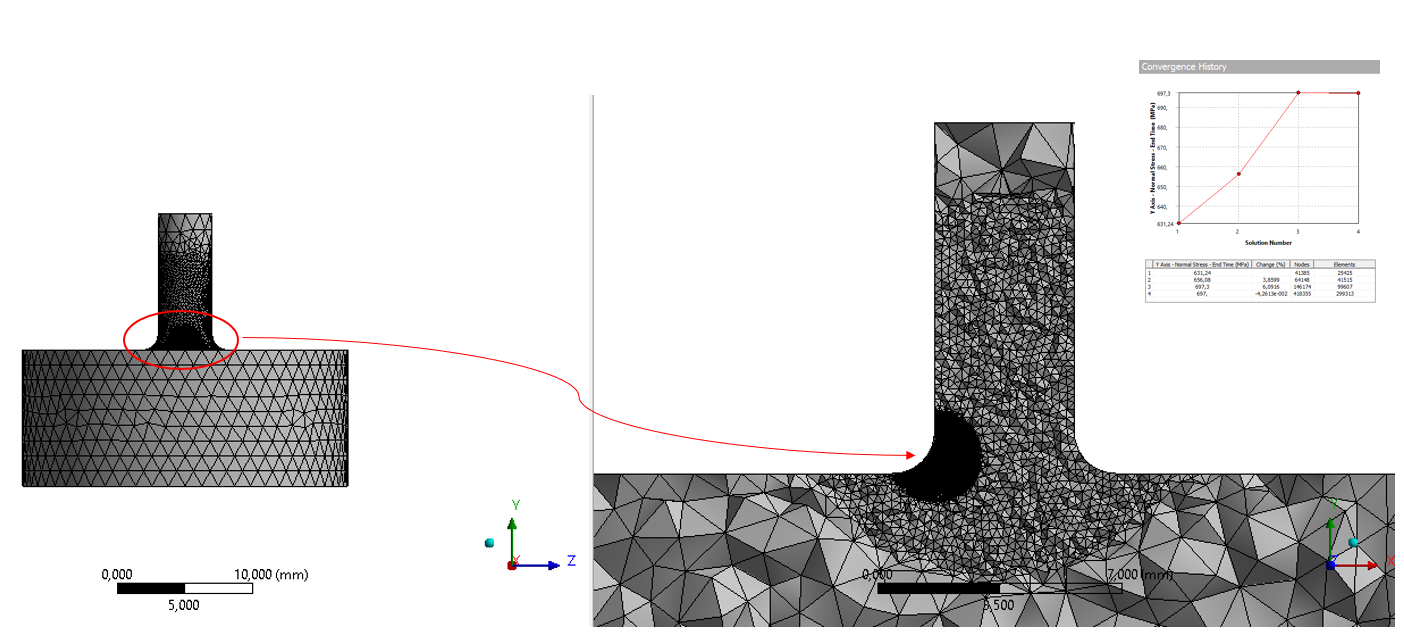
\includegraphics[width=0.8\textwidth]{pictures/CW42_3}
	\end{figure}
	\centering Tetrahedral mesh used. A mesh study with 4 levels of refinement was performed based on the maximum normal stress to assure convergence of the results obtained.
\end{frame}

\begin{frame}
  \frametitle{Review CW 42 - Boundary Conditions}
	\begin{figure}
		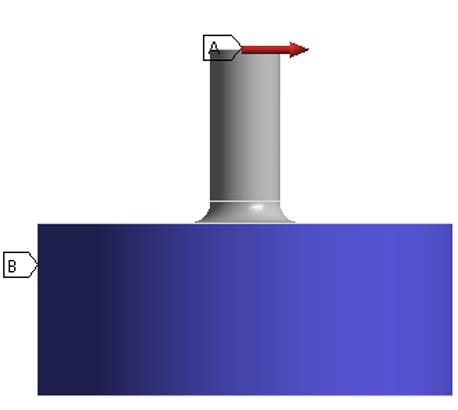
\includegraphics[width=0.5\textwidth]{pictures/CW42_4}
	\end{figure}
	\centering Simple boundary conditions used. Lateral force: 300N. Fixed base. Number of cycles for fatigue calculation: 10000 cycles with full reversal.
\end{frame}

\begin{frame}
  \frametitle{Review CW 42 - Stress Results Sample}
	\begin{figure}
		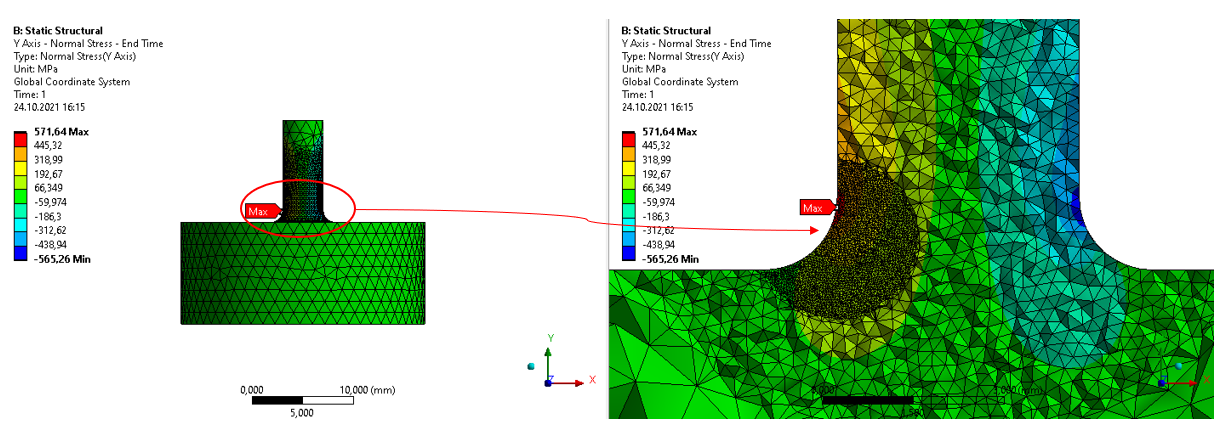
\includegraphics[width=0.9\textwidth]{pictures/CW42_5}
	\end{figure}
	\centering Representative normal stress results for one of the considered lengths. Note concentration of stress on root of cantilever beam.
\end{frame}

\begin{frame}
  \frametitle{Review CW 42 - Sections for Damage Calculation}
	\begin{figure}
		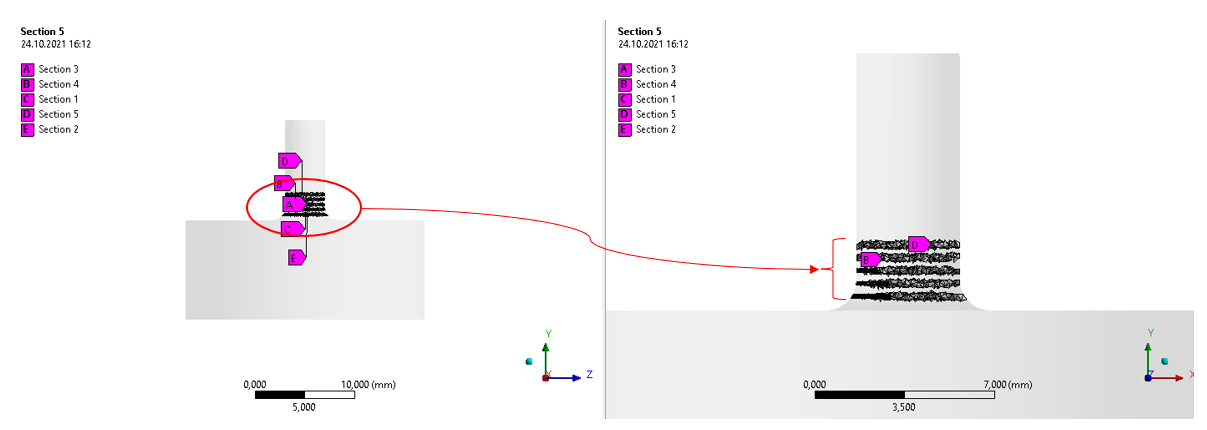
\includegraphics[width=0.9\textwidth]{pictures/CW42_6}
	\end{figure}
	\centering Cross-sections where damage is calculated for each "implant" length and then accumulated for all lengths considered.
\end{frame}

\begin{frame}
  \frametitle{Review CW 42 - Damage Calculation}
	\begin{figure}
		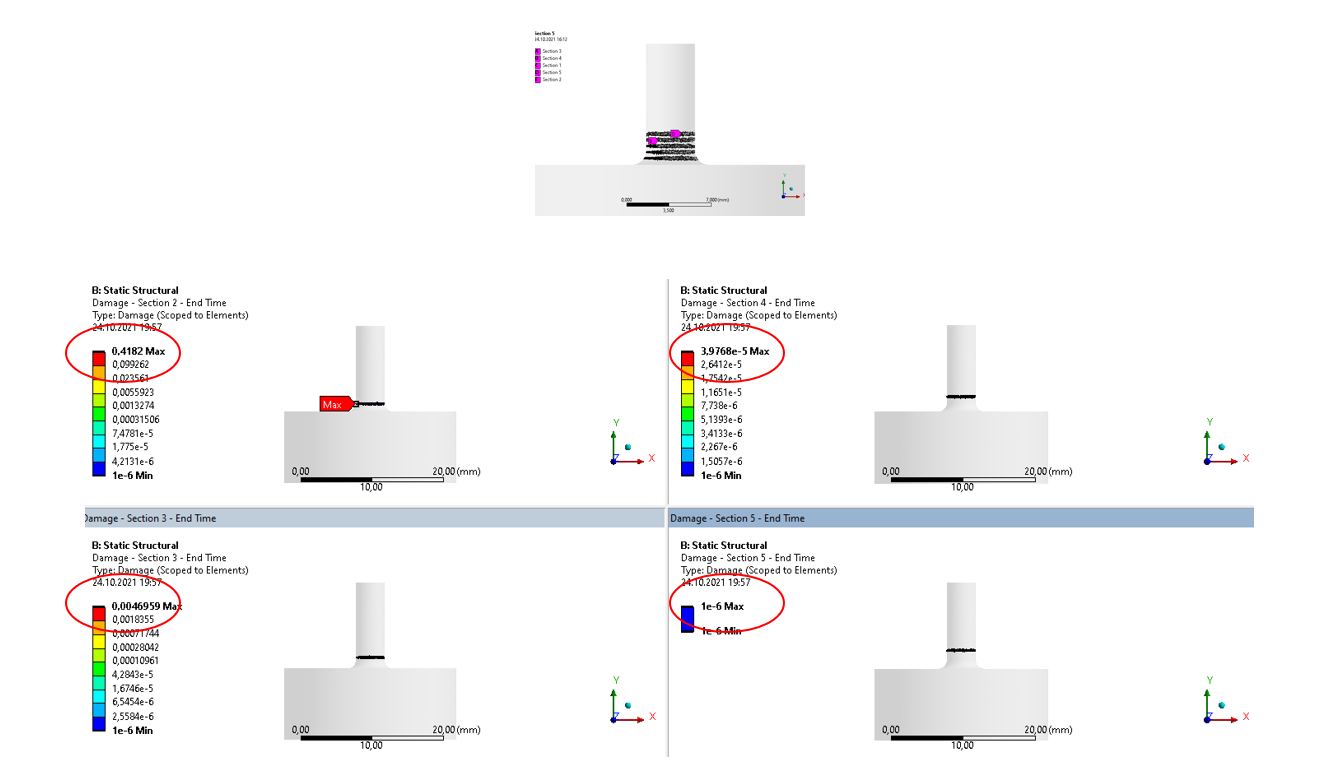
\includegraphics[width=0.5\textwidth]{pictures/CW42_7}
	\end{figure}
	Example of damage calculated for each section for a specific length. Damage calculated as proportion of applied cycles (i.e., 10000 cycles) to maximum allowable number of cycles for the calculated stress value (stress value from Ansys simulation and max allowable number of cycles from SN curve).
\end{frame}

\begin{frame}
  \frametitle{Review CW 42 - Damage Summation}
	\begin{figure}
		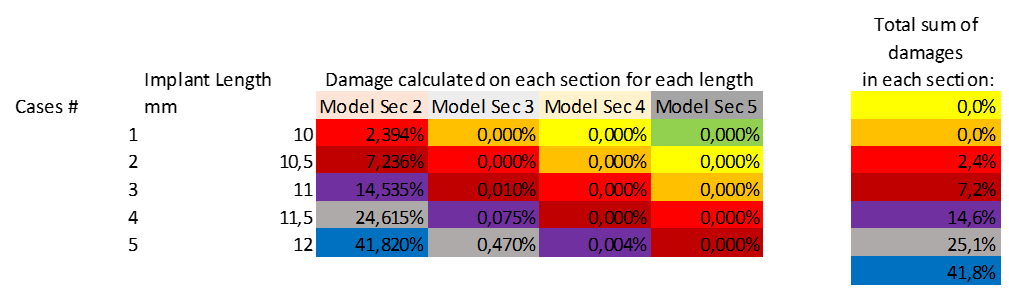
\includegraphics[width=0.6\textwidth]{pictures/CW42_8}
	\end{figure}
	Damage summation of all calculated damages at each section considering a progressing change of length of the cantilever beam (i.e., representing in a very simple manner what occurs in an implant during advancing peri-implantitis).
	Basically, the highest damage was found for the longest beam at the cross-section farthest away from the force application point (blue cell). Even though for other sections the total damage was accumulated for various lengths (other colours), it still did not compensate the higher stress for the longest beam.
\end{frame}


% ------------------------------------------------------------
% --------------------------------------------------- Slide --
\subsection{CW 43}
% ------------------------------------------------------------
% ------------------------------------------------------------
\begin{frame}
  \frametitle{Outlook CW 43}
	\begin{itemize}
		\item Start to develop fatigue calculation for more relevant case. Consider different cases length due to peri-implantitis and accumulate fatigue damage. 
		\item The idea is to basically combine the results and approches shown in:
		\begin{itemize}
		\item Calendar Week 32 (implant/bone geometry and boundary conditions as in Kitamura2004).
		\item Calendar Week 35 (automatic generation of bone support change via script).
		\item Calendar Week 42 (fatigue calculation and damage summation as just shown in this presentation).
	\end{itemize}		
		\item Prepare presentation for discussion with Prof.Dr. Stiesch and Dr. Greuling at MHH.

	\end{itemize}
\end{frame}
% --------------------------------------------------- Slide --

